\documentclass{article}
\usepackage{amsmath}
\usepackage{amssymb}
\usepackage[pdftex]{graphicx}
\usepackage[framed,numbered,autolinebreaks,useliterate]{mcode}
\lstset{breakatwhitespace=false}

\pdfpagewidth 8.5in
\pdfpageheight 11in
\topmargin -1in
\headheight 0in
\headsep 0in
\textheight 8.5in
\textwidth 6.5in
\oddsidemargin 0in
\evensidemargin 0in
\headheight 50pt
\headsep 0in
\footskip .75in

\title{STA 601 - Homework 8}
\author{Kedar Prabhudesai}
\date{September 27, 2013}

\begin{document}
\maketitle

\noindent {\Large\underline{\textbf{Missing Data:}}}\\

\noindent To simulate rejecting $p\%$ of data, I created a matrix of random values from $U[0,1]$ and ran a threshold of $p\%$ to get a random indicator matrix $O_{ij}$. I also made sure that for a given sample we have at least one value present. Using this approach I got a rejection percentage close to $p\%$.\\

\noindent This can be summarized as follows:
\begin{itemize}
\item $O_{ij} \in [0,1]$, $i = 1,2,\ldots,100$, $j = 1,2.$
\item If $O_{ij} \leq p/100 = 1$, else 0.
\item 1: Reject Data, 0: Keep Data.
\item Make sure that, $\forall i$ at least one $j$ is present.\\
\end{itemize}

\noindent {\Large\underline{\textbf{Gibbs Sampling:}}}\\
\begin{itemize}
\item Priors for $\theta$ and $\Sigma:$\\
$\mu \sim \mathcal{N}_2\left(\mu_0,\Lambda_0\right).$ $\mu_0 = \left(\begin{matrix}0.2\\0.2\end{matrix}\right)$, $\Lambda_0 = \left(\begin{matrix}1.25 & 0.6\\0.6 & 1.25\end{matrix}\right)$\\
$\Sigma \sim$ Inverse-Wishart$\left(\nu_0,S_0^{-1}\right).$ $\nu_0 = 4$, $S_0 = \left(\begin{matrix}1.2 & 0.4\\0.4 & 1.2\end{matrix}\right).$

\item Missing Data: We know that our data is drawn from a Bivariate Normal. We can partition each sample as $\{y_{obs},y_{miss}\}$

\item Gibbs Sampler: Given the starting values of $\{\Sigma^{(0)},y_{miss}^{(0)}=2\}$, we generate $\{\theta^{(s+1)},\Sigma^{(s+1)},y_{miss}^{(s+1)}\}$, as follows:
\begin{itemize}
\item $\theta^{(s+1)} \sim p(\theta|y_{obs},y_{miss}^{(s)},\Sigma^{(s)})$
\item $\Sigma^{(s+1)} \sim p(\Sigma|y_{obs},y_{miss}^{(s)},\theta^{(s+1)})$
\item $y_{miss}^{(s+1)} \sim p(y_{miss}|y_{obs},\theta^{(s+1)},\Sigma^{(s+1)})$\\
\end{itemize}

\pagebreak

\item Full Conditionals:
\begin{itemize}
\item Update $\bar{y}$
\item $\theta^{(s+1)} \mid y_{obs},y_{miss}^{(s)},\Sigma^{(s)} \sim \mathcal{N}_2\left[\left(\frac{n\Sigma^{(s)-1}\bar{y}+\Lambda_0^{-1}\mu_0}{n\Sigma^{(s)-1}+\Lambda_0^{-1}}\right),\left(n\Sigma^{(s)-1}+\Lambda_0^{-1}\right)^{-1}\right]$
\item $\Sigma^{(s+1)} \mid y_{obs},y_{miss}^{(s)},\theta^{(s+1)} \sim IW\left[\nu_0+n,\left(S_0+S_{\theta}\right)^{-1}\right],S_{\theta} = \sum_{i=1}^{n}(y_i-\theta^{(s+1)})(y_i-\theta^{(s+1)})'$\\
\item $y_{miss}^{(s+1)} \mid y_{obs},\theta^{(s+1)},\Sigma^{(s+1)} \sim \mathcal{N}\left(\theta_{b|a}^{(s+1)},\Sigma_{b|a}^{(s+1)}\right)$\\
$\theta_{b|a}^{(s+1)} = \theta_{b}^{(s+1)} + \Sigma_{b,a}^{(s+1)}\left(\Sigma_{a,a}^{(s+1)}\right)^{-1}\left(y_{a}-\theta^{(s+1)_{a}}\right)$\\
$\Sigma_{b|a}^{(s+1)} = \Sigma_{b,b}^{(s+1)} - \Sigma_{b,a}^{(s+1)}\left(\Sigma_{a,a}^{(s+1)}\right)^{-1}\Sigma_{a,b}^{(s+1)}$, \\
where, $b$ is the index of 'Data Missing' and $a$ is index of 'Data Present'.\\
\end{itemize}

\noindent {\Large\underline{\textbf{Results:}}} \\

Gibbs Samples = 10000, Burn-In = 1000. Given here are estimates of $E(\theta_1)$ and $E(\theta_2)$ with their 95\% Credible Intervals. We see that as the \% of rejected data increases, our estimate of mean is less accurate and has a larger credible interval. Note that $0\%$ point represents no data was rejected.\\

\begin{left}
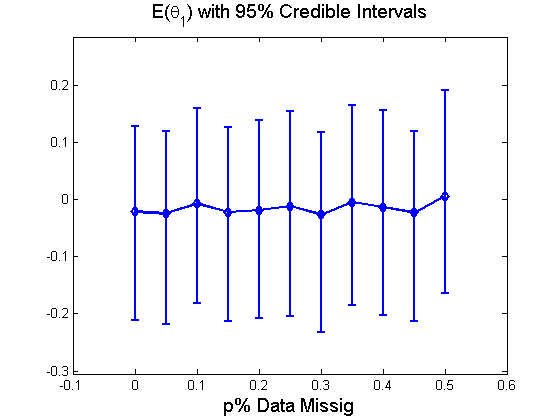
\includegraphics[scale=0.5]{Theta1_Conf.png}
\end{left}
\begin{right}
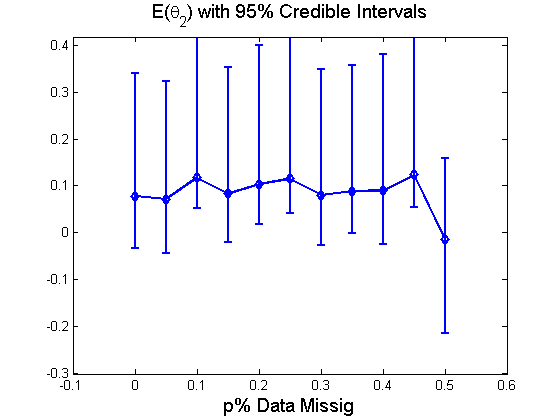
\includegraphics[scale=0.5]{Theta2_Conf.png}\\
\end{right}

\pagebreak
\noindent {\Large\underline{\textbf{Complete Case Analysis:}}} \\

For this we reject all samples which contain missing data. By doing this our estimate wanders even more about the true estimate and the intervals are much bigger than when we impute the missing data.\\

\begin{left}
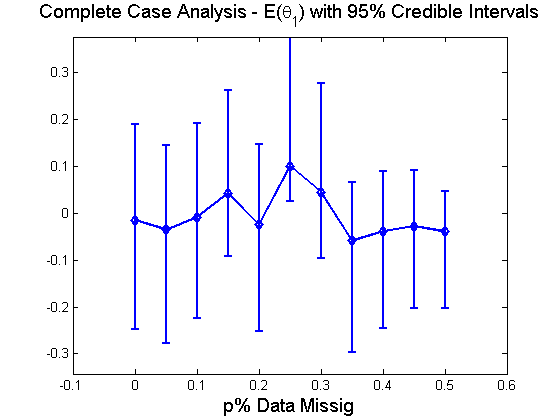
\includegraphics[scale=0.5]{CCTheta1_Conf.png}
\end{left}
\begin{right}
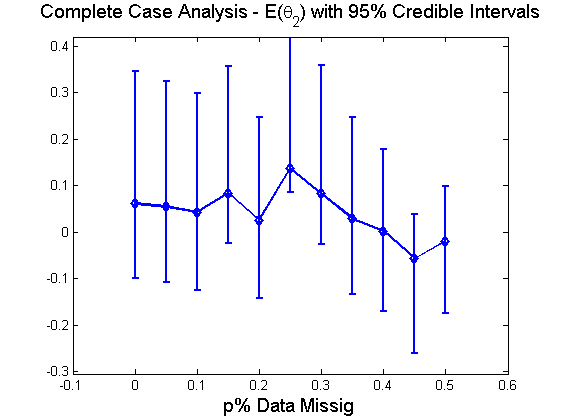
\includegraphics[scale=0.5]{CCTheta2_Conf.png}\\
\end{right}

\noindent 

\end{itemize}

\pagebreak
\noindent {\Large\underline{\textbf{Appendix:}}}\\
\lstinputlisting{C:/Users/ksp6/Documents/Classes/2013-Fall/STA601-BayesAndModStats/homeworks/hw8/hw8.m}

\end{document}